In the section, the wristband layer is described in greater detail in terms of its subsystems.
% In this section, the layer is described in some detail in terms of its specific subsystems. Describe each of the layers and its subsystems in a separate chapter/major subsection of this document. The content of each subsystem description should be similar. Include in this section any special considerations and/or trade-offs considered for the approach you have chosen.


\subsection{Micro-controller}
This subsystem is responsible for controlling the overall functioning of the device.

\begin{figure}[h!]
	\centering
 	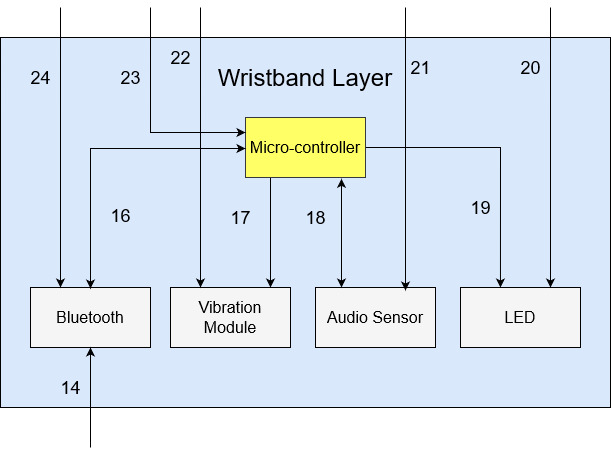
\includegraphics[width=0.60\textwidth]{images/wristband-micro.jpg}
 \caption{Wristband Micro-controller Subsystem diagram}
\end{figure}

\subsubsection{Assumptions}
It is assumed that all modules are properly connected and working. It is also assumed that there is power in the system.

\subsubsection{Responsibilities}
The micro-controller is connected to the Bluetooth, vibration, audio sensor, and LED modules. Once a Bluetooth signal is received to vibrate, the micro-controller sends a signal to the vibration module to vibrate in a specific pattern. Additionally, once the audio sensor detects a certain decibel level, the micro-controller sends a signal to the LED to be a certain color.

\subsubsection{Subsystem Interfaces}

\begin {table}[H]
\caption {Micro-Controller interfaces} 
\begin{center}
    \begin{tabular}{ | p{1cm} | p{6cm} | p{3cm} | p{3cm} |}
    \hline
    ID & Description & Inputs & Outputs \\ \hline
    16 & Bluetooth - Micro-Controller & Instructions for Vibrations & Signals \& Instructions to Operate \\ \hline
    17 & Vibration Module - Micro-Controller & N/A & Signals to Vibrate \\ \hline
    18 & Audio Sensor - Micro-Controller & Decibel Levels & Signals to Operate \\ \hline
    19 & LED - Micro-Controller & N/A & Signals \& Colors to Light \\ \hline
    23 & Power - Micro-Controller & Power (W) & N/A \\ \hline
%    \#xx & Description of the interface/bus & \pbox{3cm}{input 1 \\ input 2} & \pbox{3cm}{output 1}  \\ \hline
    %\#xx & Description of the interface/bus & \pbox{3cm}{N/A} & \pbox{3cm}{output 1}  \\ \hline
    \end{tabular}
\end{center}
\end{table}

\subsection{Bluetooth}
The Bluetooth subsystem is responsible for connecting to the user's phone and receiving signals via the Cerberus app.

\begin{figure}[h!]
	\centering
 	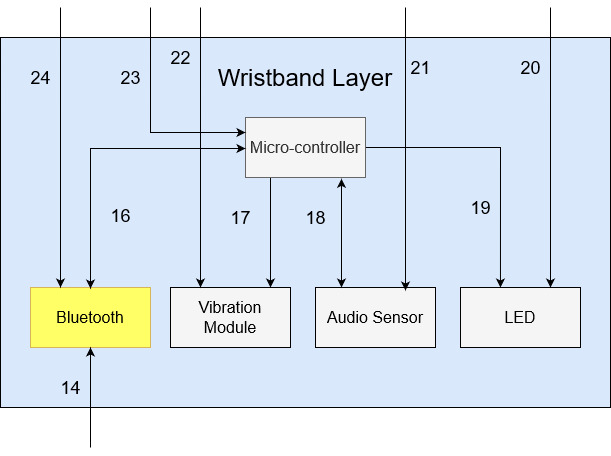
\includegraphics[width=0.60\textwidth]{images/wristband-bluetooth.jpg}
 \caption{Wristband Bluetooth Subsystem diagram}
\end{figure}

\subsubsection{Assumptions}
It is assumed that the Bluetooth module is functioning properly. It is also assumed that wristband is charged and the Bluetooth module is receiving power from the power layer.

\subsubsection{Responsibilities}
The Bluetooth module must be able to connect to devices capable of receiving Bluetooth signals. Upon connection, it must stay connected to the device. Once connected to the device, when it receives information from the Cerberus app such as notifications and vibration signals, it will send the information to the micro-controller.

\subsubsection{Subsystem Interfaces}

\begin {table}[H]
\caption {Bluetooth interfaces} 
\begin{center}
    \begin{tabular}{ | p{1cm} | p{6cm} | p{3cm} | p{3cm} |}
    \hline
    ID & Description & Inputs & Outputs \\ \hline
    14 & Bluetooth to Phone App & Vibration Instructions & Connectivity Signals \\ \hline
    16 & Bluetooth - Micro-controller & Instructions & Signals to Vibrate \\ \hline
    24 & Power to Bluetooth & Power (W) & N/A \\ \hline
    %\#xx & Description of the interface/bus & \pbox{3cm}{input 1 \\ input 2} & \pbox{3cm}{output 1}  \\ \hline
    %\#xx & Description of the interface/bus & \pbox{3cm}{N/A} & \pbox{3cm}{output 1}  \\ \hline
    \end{tabular}
\end{center}
\end{table}

\subsection{Audio Sensor}
The audio sensor detects decibel levels so the LED can be changed to a specific color.

\begin{figure}[h!]
	\centering
 	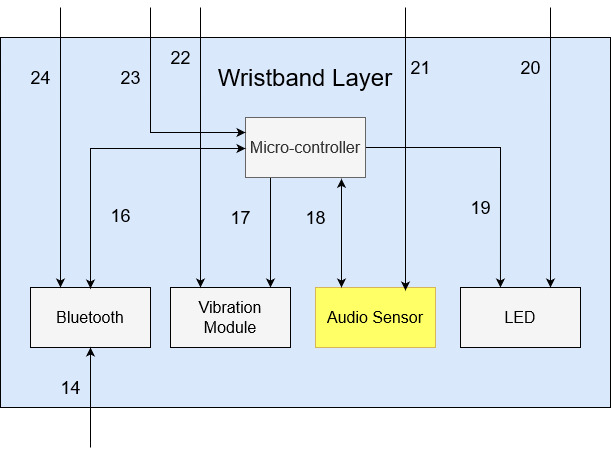
\includegraphics[width=0.60\textwidth]{images/wristband-audio.jpg}
 \caption{Wristband Audio Sensor Subsystem diagram}
\end{figure}

\subsubsection{Assumptions}
It is assumed that the module is functional and there is power in the power layer.

\subsubsection{Responsibilities}
The audio sensor is responsible for detecting the decibel level in the area the sensor is in. It is responsible for sending the audio readings to the micro-controller.

\subsubsection{Subsystem Interfaces}

\begin {table}[H]
\caption {Audio Sensor interfaces} 
\begin{center}
    \begin{tabular}{ | p{1cm} | p{6cm} | p{3cm} | p{3cm} |}
    \hline
    ID & Description & Inputs & Outputs \\ \hline
    18 & Bluetooth - Micro-controller & Setup Instructions & Audio \\ \hline
    21 & Power to Audio Sensor & Power (W) &  N/A \\ \hline
    %\#xx & Description of the interface/bus & \pbox{3cm}{input 1 \\ input 2} & \pbox{3cm}{output 1}  \\ \hline
    %\#xx & Description of the interface/bus & \pbox{3cm}{N/A} & \pbox{3cm}{output 1}  \\ \hline
    \end{tabular}
\end{center}
\end{table}

\subsection{LED}
This subsystem lights up according to the decibel level in the room.

\begin{figure}[h!]
	\centering
 	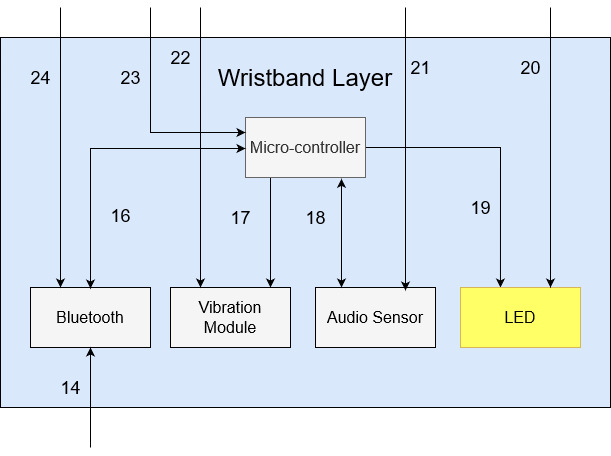
\includegraphics[width=0.60\textwidth]{images/wristband-led.jpg}
 \caption{Wristband Bluetooth Subsystem diagram}
\end{figure}

\subsubsection{Assumptions}
It is assumed that there is power in the system. It is also assumed that the audio sensor subsystem is operating properly.

\subsubsection{Responsibilities}
This subsystem is responsible for receiving the room's current decibel level from the micro-controller. It then lights up red if the room is loud, yellow if some noise, but not much, and green if quiet.

\subsubsection{Subsystem Interfaces}

\begin {table}[H]
\caption {LED interfaces} 
\begin{center}
    \begin{tabular}{ | p{1cm} | p{6cm} | p{3cm} | p{3cm} |}
    \hline
    ID & Description & Inputs & Outputs \\ \hline
    19 & Power to LEDs & Power (W) &  N/A \\ \hline
    20 & LED - Micro-controller & Instructions & N/A \\ \hline
    %\#xx & Description of the interface/bus & \pbox{3cm}{input 1 \\ input 2} & \pbox{3cm}{output 1}  \\ \hline
    %\#xx & Description of the interface/bus & \pbox{3cm}{N/A} & \pbox{3cm}{output 1}  \\ \hline
    \end{tabular}
\end{center}
\end{table}

\subsection{Vibration Module}
This subsystem is responsible for vibrating various patterns depending on what information is received from the micro-controller.

\begin{figure}[h!]
	\centering
 	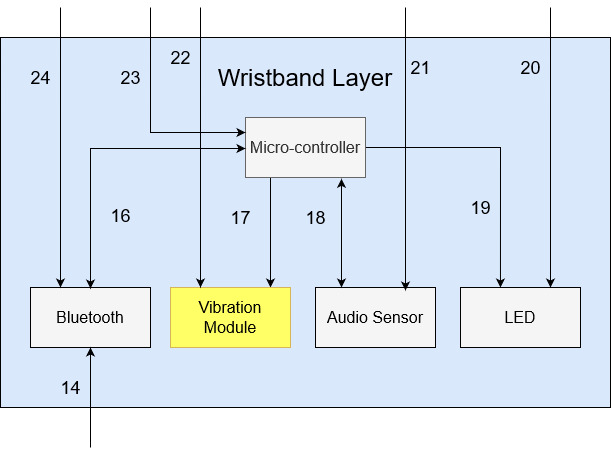
\includegraphics[width=0.60\textwidth]{images/wristband-vibration.jpg}
 \caption{Wristband Vibration Subsystem diagram}
\end{figure}

\subsubsection{Assumptions}
It is assumed that there is power in the system. It is also assumed that the Bluetooth module and micro-controller are functioning properly.

\subsubsection{Responsibilities}
This subsystem is responsible for receiving signals from the micro-controller to vibrate, causing the vibration motor to vibrate in specific patterns.

\subsubsection{Subsystem Interfaces}

\begin {table}[H]
\caption {Vibration Module interfaces} 
\begin{center}
    \begin{tabular}{ | p{1cm} | p{6cm} | p{3cm} | p{3cm} |}
    \hline
    ID & Description & Inputs & Outputs \\ \hline
    17 & Power to Vibration Motor & Power (W) &  N/A \\ \hline
    22 & Vibration Motor - Micro-controller & Instructions & N/A \\ \hline
    %\#xx & Description of the interface/bus & \pbox{3cm}{input 1 \\ input 2} & \pbox{3cm}{output 1}  \\ \hline
    %\#xx & Description of the interface/bus & \pbox{3cm}{N/A} & \pbox{3cm}{output 1}  \\ \hline
    \end{tabular}
\end{center}
\end{table}
